% ----------------------------------------------------------
% Contextualização em Humanidades
% ----------------------------------------------------------
\chapter{Contextualização em Humanidades}
\label{chap:ctx-hum}
% ----------------------------------------------------------


Nos últimos anos, houve um progresso significativo na solução de problemas desafiadores em diversos campos, utilizando algoritmos de \textit{deep reinforcement learning}. Como consequência, o RL experimentou um crescimento dramático na atenção e no interesse da comunidade científica. 
% A \textbf{Figura \ref{rl-publications-overview}} mostra o crescimento no número de publicações relacionadas à RL nos últimos 30 anos.

% \begin{figure}[h]
%   \centering
%   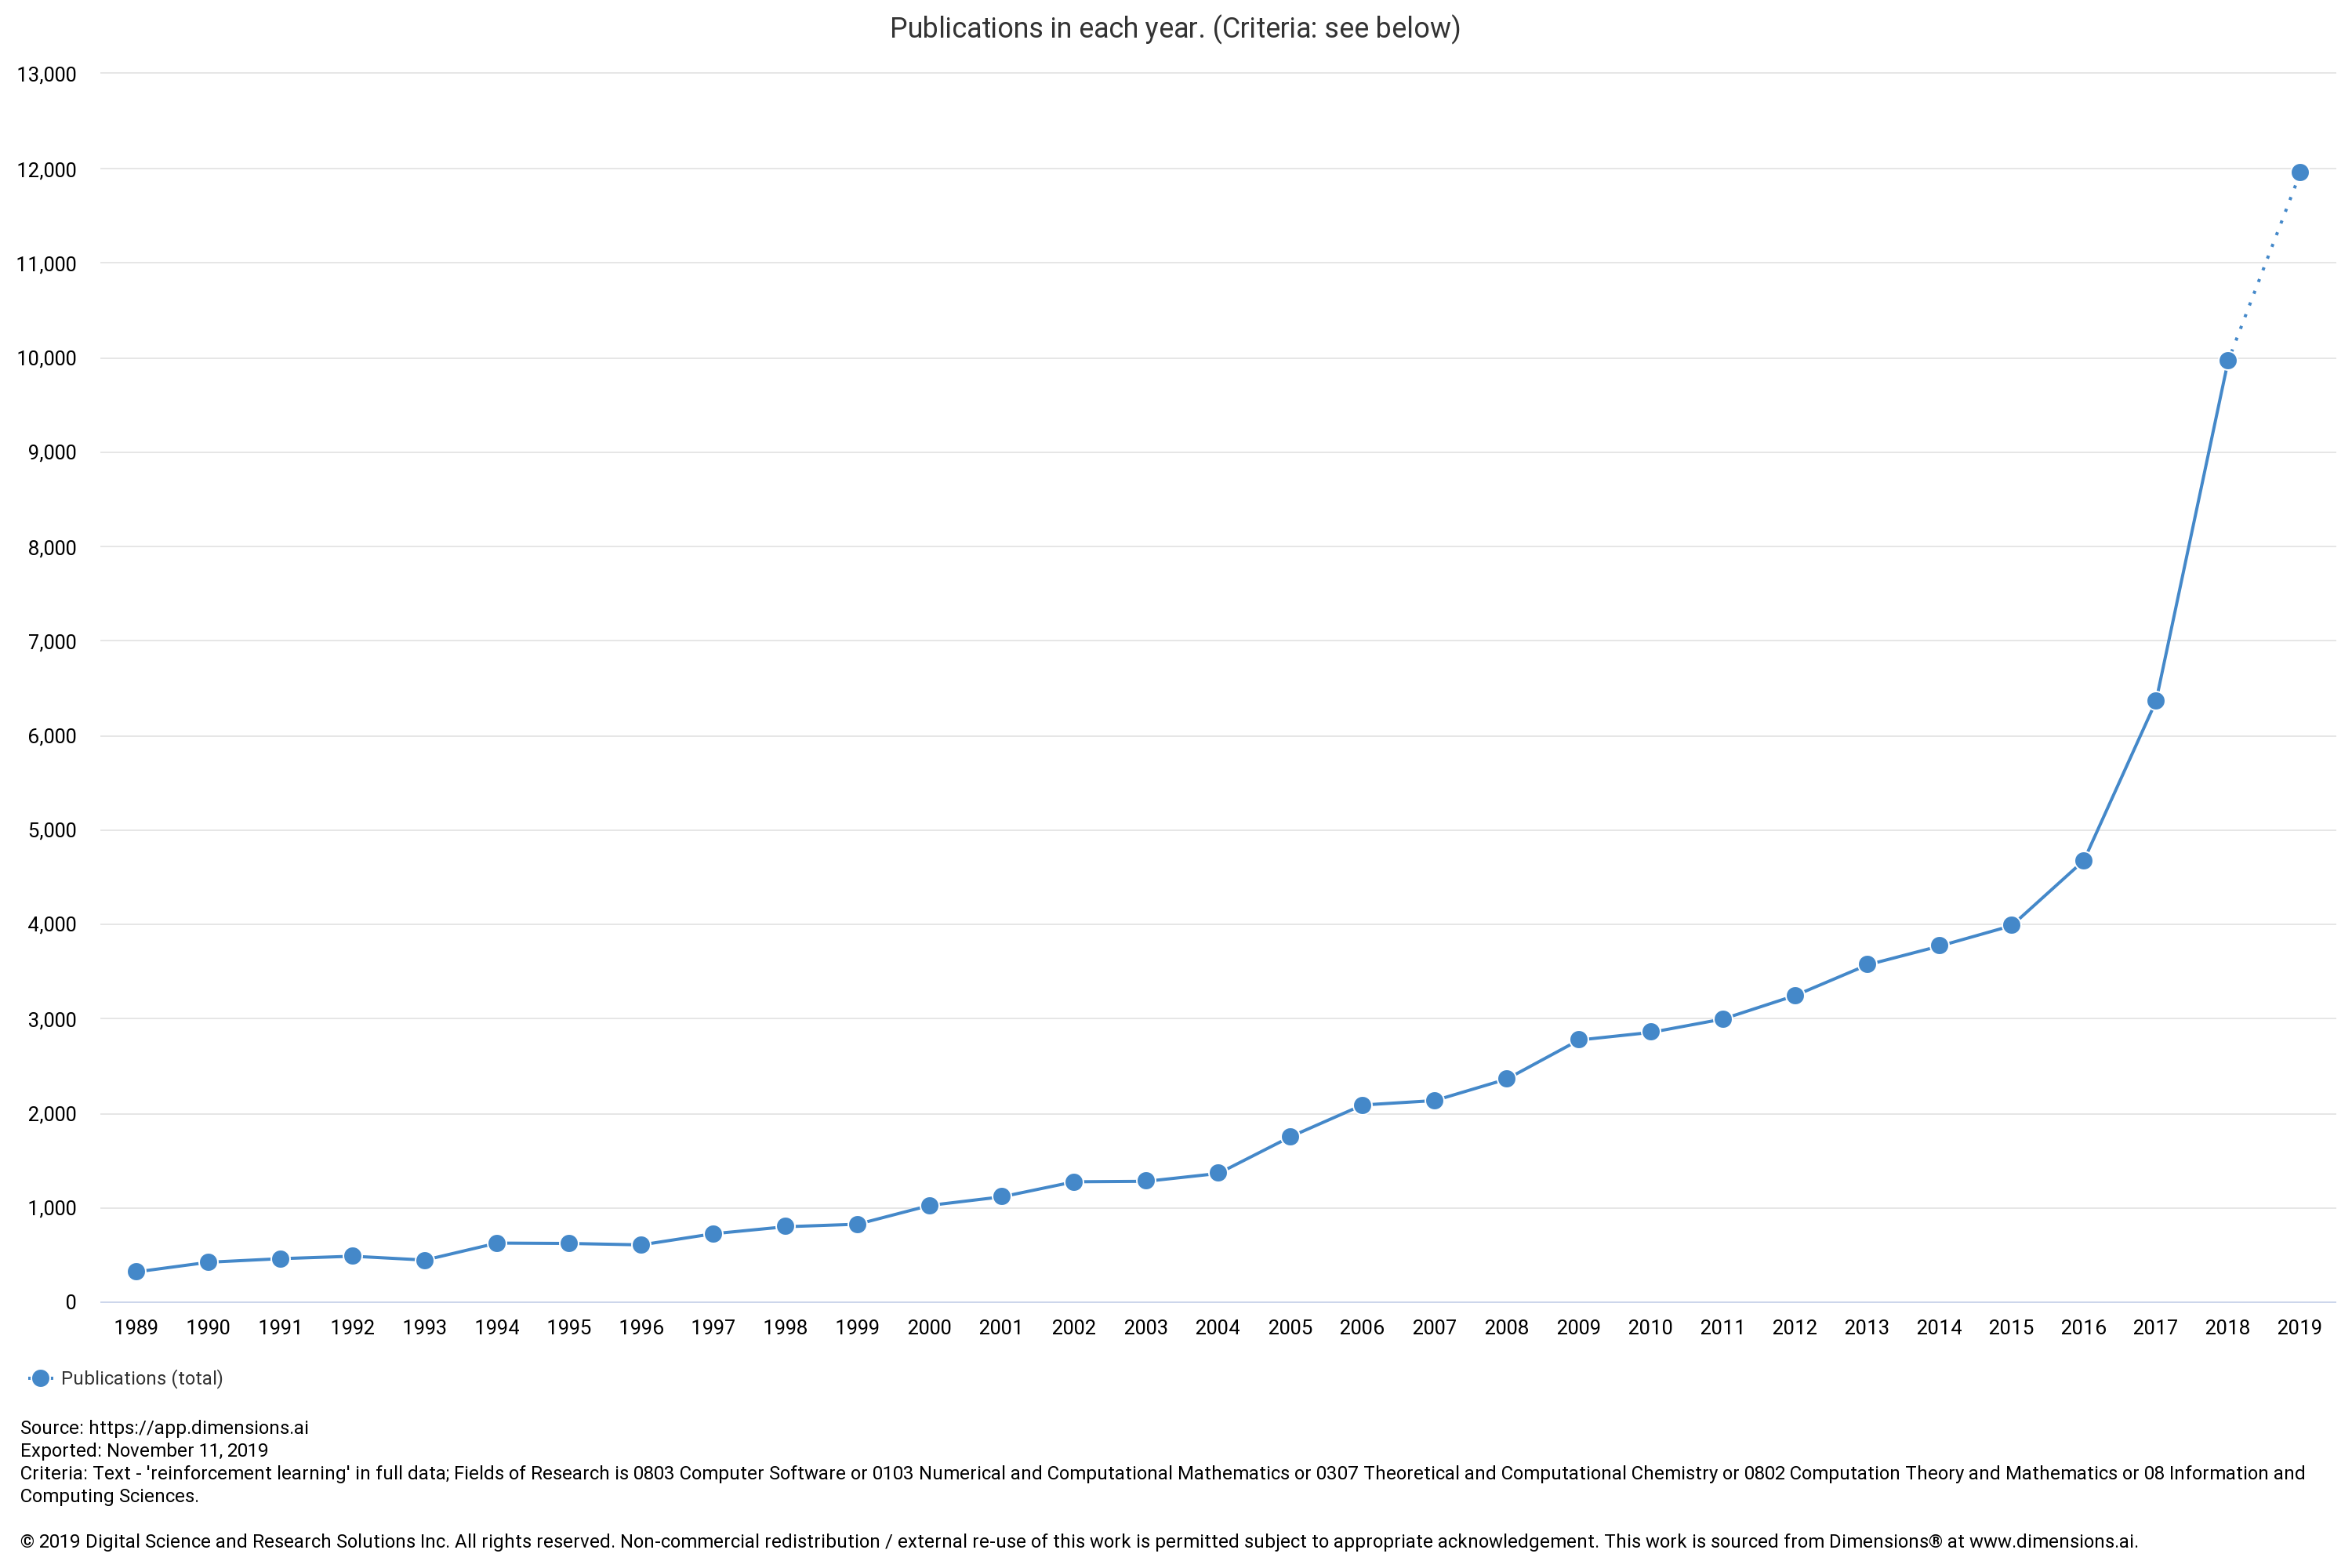
\includegraphics[width=.7 \textwidth]{conteudo/imgs/rl-publications-overview.png}
%   \caption[Crescimento do número de publicações sobre RL]{Crescimento do número de publicações sobre \textit{Reinforcement Learning.}}
%   \label{rl-publications-overview}
%  \end{figure}


Do ponto de vista econômico, são inúmeros os usos de \textit{deep learning} no mercado. Desde ferramentas que melhoram a precisão dos sensores de precipitação por satélite e concentrando-se na redução do viés e dos alarmes falsos \cite{doi:10.1175/JHM-D-15-0075.1}, à agentes que permitem que diferentes dispositivos eletrônicos interpretem dados de multimídia não estruturados e reajam de maneira inteligente aos eventos do usuário e do ambiente \cite{dl-IoT}, o DL tem se tornado cada vez mais presente e essencial para a sociedade. Grandes setores e empresas na área da tecnologia não existiriam sem o uso dessas ferramentas.

Em relação aos impactos sociais do DL podemos mencionar a sua utilização para estimar as características socioeconômicas de regiões de 200 cidades dos Estados Unidos usando 50 milhões de imagens de cenas de rua reunidas com carros do \textit{Google Street View} \cite{Gebru13108}. O DL também teve impactos em diversas áreas da ciência, desde pesquisa em física de partículas \cite{baldi:s:w:2015}, à medicina \cite{nassif:speech-rec:2019}.

É interessante ressaltar que apesar de todos os benefícios oferecidos pela IA, alguns indivíduos notáveis como o famoso físico Stephen Hawking, e o líder da Tesla e da SpaceX Elon Musk, sugerem que a IA pode ser potencialmente muito perigosa. De fato, existem muitos aplicativos de IA que tornam nossa vida cotidiana mais conveniente e eficiente. São os aplicativos de IA que desempenham um papel crítico para garantir a segurança que Musk, Hawking e outros estavam preocupados quando proclamaram sua hesitação sobre a tecnologia. Por exemplo, se a IA for responsável por garantir a operação de nossa rede elétrica, de uma usina nuclear ou outro sistema de alto risco, e a IA for invadida ou tiver seus objetivos desalinhados com os nossos, isso poderá resultar em danos enormes \cite{Marr:AI-Danger}. 
% \clearpage

Apesar de todo o medo ao redor dessa nova tecnologia, muitos argumentam que os mesmos são exagerados e que os benefícios oferecidos são muito maiores que os potenciais riscos, desde que sejam gerenciados adequadamente. O crescimento de pesquisas em DRL revelam seu grande potencial e benefícios para a sociedade. Reproduzir e comparar os trabalhos existentes existente e julgar com precisão as melhorias oferecidas por novos métodos é vital para sustentar esse progresso. 

\clearpage
No contexto de jogos digitais, treinar um agente para superar os jogadores humanos e otimizar sua pontuação pode nos ensinar como otimizar processos diferentes em uma variedade de subcampos diferentes e intrigantes \cite{comi:teach:AI:DRL:2018}. Os impactos econômicos e sociais que essas técnicas podem oferecer são diversos. 

Situações do mundo real são muitas vezes complexas e apresentam problemas com um número muito grande de variáveis. Para tais problemas, encontrar a melhor solução pode ser um desafio muito grande para algoritmos de otimização tradicionais. Uma vez que se tenha um sistema capaz de aprender e elaborar estratégias para diferentes cenários, é fácil modelar problemas que possam ser resolvidos pelo mesmo. No caso, uma IA que possa aprender a jogar e a otimizar estratégias para maximizar a pontuação de um jogo, pode ser aplicada em um jogo que simule uma situação real e encontrar a melhor resposta ou solução para um dado problema. 

Imagine, por exemplo, um jogo que simule o trânsito em uma cidade, e a pontuação desse jogo é calculada de acordo com a elaboração das rotas de ônibus, as quais devem alcançar o maior número de áreas da cidade e minimizar o tempo de cada trajeto. A IA proposta seria, idealmente, capaz de encontrar a melhor organização possível dessas rotas. Na área da biomedicina e química, poderíamos modelar um jogo que simule o comportamento de uma célula cancerígena, e a IA teria o objetivo de encontrar o tratamento mais efetivo para a doença. Um jogo que simule condições extremas de temperaturas, ambiente e terreno, poderia ser aplicado ao sistema e a IA poderia propor a modelagem das máquinas que iriam se adaptar melhor à dadas condições. Essas máquinas, por sua vez, poderiam ser utilizadas em diversas expedições espaciais ou de alta profundidade, por exemplo. O sistema proposto, portanto, poderia idealmente ser aplicado para quaisquer cenários ou jogos, os quais podem ser modelados para serem mais ou menos complexos, de forma a melhor atender a necessidade do usuário. 


Em resumo, o DL já é utilizado com sucesso em diversas áreas da ciência, otimizando e solucionando diferentes problemas. Ao propor um sistema que seja flexível e capaz de se adaptar à diferentes cenários, seria capaz de unificar muitas dessas ferramentas em uma única. A mesma ferramenta poderia ser aplicada nas diferentes situações mencionadas anteriormente e propor soluções para inúmeros problemas, melhorar produtos já existentes e otimizar processos no mundo real.



